\vspace{-1em}
\section{Formalization of the graph mining problem}\label{sec:formalization}
\subsection{Patterns}
We start with a comprehensive formal definition of the graph mining problem.
First, we will assume the existence of two finite, sufficiently large sets: a set $V_{U}$ consisting of vertices, and a set $L$ of possible labels for those vertices.

\begin{definition}
A labeled graph \graph{G} is a tuple $\triple{V,E,l}$ where $V$ is the set of vertices in the graph, $E$ is a binary predicate on $V$ that represents the set of (directed) edges and $l$ is a unary function from $V$ to $L$. 
%We call $V_{\graph{G}}$ the restriction of $V$ to vertices actually present in edges of $\graph{G}$.
\end{definition}
\vspace{-1.5em}
\begin{definition}
A graph $\graph{G} = \triple{V,E,l}$ is \emph{connected} iff for each pair of vertices $v$ and $v'$ in $V_{\graph{G}}$, there exists an edge $\pair{v,v'} \in E$ or there exists a sequence $v, v_{1} \ldots v_{n}, v'$ such that there exist edges $\pair{v,v_{1}}$, $\pair{v_{i},v_{i+1}}$ and $\pair{v_{n},v'} \in E$, where $1 \leq i \leq n-1$.
\end{definition}

\begin{definition}
A graph homomorphism $f$ from a labeled graph $\graph{G} = \triple{V,E,l}$ to a labeled graph $\graph{G}' = \triple{V',E',l'}$ is an injective mapping $f$ : $V \rightarrow V'$ from vertices of $\graph{G}$ to vertices of $\graph{G'}$ such that:
\begin{compactitem}
\item $\forall v \in V : l(v) = l(f(v))$ (the mapping respects labelings), and
\item $\forall u,v \in V : \pair{u,v} \in E \implies \pair{f(u),f(v)} \in E'$ (the mapping preserves edges).
\end{compactitem}
If a graph homomorphism from graph $\graph{G}$ to $\graph{G'}$ exists we say $\graph{G}$ is \emph{homomorphic} with $\graph{G'}$.
\end{definition}

\begin{definition} \textbf{Graph Mining}
\label{def:gm2}
Given a sufficiently large set of vertices $V$ and labels $L$, two sets $\graphset{G}_{+}$ and $\graphset{G}_{-}$ of positive, respectively negative example graphs over $V$ and $L$ and a graph $\graph{T}$ over $V$ and $L$ called the template,
%which consist of an edge relation, 
we look for a 
%(set $\graphset{P}$ of) \todo{cleanly extend this definition to multiple graphs, or separate the single and multiple pattern case again}
graph \graph{P} represented by tuple $\triple{E_{\graph{P}}, l_{\graph{P}}}$ such that:
%for at least $N_{+}$ of the triples $\triple{ E, l, C}$ with $C=Pos$, and for at most $N_{-}$ of such triples with $C=Neg$, there exists a function $f$ s.t. $\forall u,v \in V, \pair{u,v} \in E_{p} \implies \pair{f(u),f(v)} \in E$ and $\forall v \in V : l_{p}(v) = l(f(v))$.
\vspace{0.5em}
\begin{compactitem}
\item $\graph{P}$ is a \emph{connected} subgraph of $\graph{T}$,
\item $\graph{P}$ is homomorphic with at least $N_{+}$ positive examples
$\graph{G}_{+} \in \graphset{G}_{+}$,
\item $\graph{P}$ is homomorphic with at most $N_{-}$ negative examples $\graph{G}_{-} \in \graphset{G}_{+}$.
%$\#\Big\lbrace \triple{E,l,pos} \in \graphset{G} \; | \; \exists f : \text{f is a homomorphism from \graph{P} to \triple{E,l,pos}} \Big\rbrace \geq N_{+}$,
%\item $\#\Big\lbrace \triple{E,l,neg} \in \graphset{G} \; | \; \exists f : \text{f is a homomorphism from \graph{P} to \triple{E,l,neg}} \Big\rbrace \leq N_{-}$.
\end{compactitem}
\end{definition}
%\begin{definition}
%\label{def:GM1}
%Given a pair $\triple{\graphset{E}_{+},\graphset{E}_{-}}$ consisting of a set of \emph{positive} and \emph{negative} examples of \emph{labeled graphs} respectively, 
%and a graph $\graph{T}$ called the template,
%\emph{Graph mining} is the problem of finding a pattern $\graph{P}$ which is
%\begin{compactitem}
%\item a \emph{connected labeled subgraph of $\graph{T}$},
%\item \emph{homomorphic} with at least $N_{+}$ positive examples $\graph{E}_{+} \in \graphset{E}_{+}$, while being homomorphic with at most $N_{-}$ negative examples $\graph{E}_{-} \in \graphset{E}_{-}$. 
%\end{compactitem}
%%This pattern $\graph{P}$ must be \emph{homomorphic} with at least $N_{+}$ positive, while being homomorphic with at most $N_{-}$ negative examples. 
%\end{definition}
We call these homomorphisms the positive (negative) homomorphisms, and the restriction on their number the positive (negative) homomorphic property, respectively. 
Note that we include the concept of a template graph to guide as well as limit the search.

\tikzstyle{vertex} = [circle, fill=black, radius=1pt, inner sep=0pt, minimum size=3pt]
\begin{figure}[h]
\captionsetup{justification=centering}
%\vspace{-0.5em}
\vspace{-2em}
  \centering
  \begin{subfigure}[b]{0.18\textwidth}
    \centering
    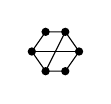
\begin{tikzpicture}[scale=.25]
      \node[vertex] (a) at (1,1) {};
      \node[vertex] (b) at (2,1) {};
      \node[vertex] (c) at (2.7,2) {};
      \node[vertex] (d) at (2,3) {};
      \node[vertex] (e) at (1,3) {};
      \node[vertex] (f) at (0.3,2) {};
      \draw (1,1) -- (2,1) -- (2.7,2) -- (2,3) -- (1,3) -- (0.3,2) -- (1,1);
      \draw (1,1) -- (2,3);
      \draw (2.7,2) -- (0.3,2);
    \end{tikzpicture}
    \caption{Positive\\Example\label{fig:pos}}
  \end{subfigure}
  ~
  \begin{subfigure}[b]{0.18\textwidth}
    \centering
    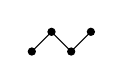
\begin{tikzpicture}[scale=.25]
      \node[vertex] (a) at (0,0) {};
      \node[vertex] (b) at (1,1) {};
      \node[vertex] (c) at (2,0) {};
      \node[vertex] (d) at (3,1) {};
      \coordinate (1) at (0,0);
      \coordinate (2) at (1,1);
      \coordinate (3) at (2,0);
      \coordinate (4) at (3,1);
      \draw (1) -- (2) -- (3) -- (4);
    \end{tikzpicture}
    \caption{Negative\\Example\label{fig:neg}}
  \end{subfigure}
  ~
  \begin{subfigure}[b]{0.18\textwidth}
    \centering
    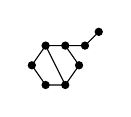
\begin{tikzpicture}[scale=.25]
      \node[vertex] (a) at (1,1) {};
      \node[vertex] (b) at (2,1) {};
      \node[vertex] (c) at (2.7,2) {};
      \node[vertex] (d) at (2,3) {};
      \node[vertex] (e) at (1,3) {};
      \node[vertex] (f) at (0.3,2) {};
      \node[vertex] (g) at (3,3) {};
      \node[vertex] (h) at (3.7,3.7) {};
      \draw (1,1) -- (2,1) -- (2.7,2) -- (2,3) -- (1,3) -- (0.3,2) -- (1,1);
      %\draw (1,1) -- (2,3);
      %\draw (2.7,2) -- (0.3,2);
      \draw (1,3) -- (2,1);
      \draw (2,3) -- (3,3) -- (3.7,3.7);
    \end{tikzpicture}
    \caption{Template\\Graph\label{fig:templ}}
  \end{subfigure}
  ~
  \begin{subfigure}[b]{0.18\textwidth}
    \centering
    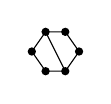
\begin{tikzpicture}[scale=.25]
       \node[vertex] (a) at (1,1) {};
       \node[vertex] (b) at (2,1) {};
       \node[vertex] (c) at (2.7,2) {};
       \node[vertex] (d) at (2,3) {};
       \node[vertex] (e) at (1,3) {};
       \node[vertex] (f) at (0.3,2) {};
          
       \draw (1,1) -- (2,1) -- (2.7,2) -- (2,3) -- (1,3) -- (0.3,2) -- (1,1);
       \draw (2,1) -- (1,3);
     \end{tikzpicture}
  \caption{\label{fig:correctcandidate}Candidate\\1}
  \end{subfigure}
  ~
  \begin{subfigure}[b]{0.18\textwidth}
    \centering
    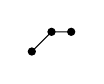
\begin{tikzpicture}[scale=.25]
      \node[vertex] (a) at (1,2) {};
      \node[vertex] (b) at (2,3) {};
      \node[vertex] (c) at (3,3) {};
      \draw (1,2) -- (2,3) -- (3,3);
    \end{tikzpicture}
    \caption{\label{fig:incorrectcandidate}Candidate\\2}
  \end{subfigure}

%  \begin{subfigure}[b]{0.24\textwidth}
%    {
%      \setcounter{subfigure}{0}
%      \renewcommand\thesubfigure{\Roman{subfigure}}
%      \centering
%      \begin{subfigure}[b]{0.24\textwidth}
%        \begin{tikzpicture}[scale=.25]
%          \node[vertex] (a) at (1,1) {};
%          \node[vertex] (b) at (2,1) {};
%          \node[vertex] (c) at (2.7,2) {};
%          \node[vertex] (d) at (2,3) {};
%          \node[vertex] (e) at (1,3) {};
%          \node[vertex] (f) at (0.3,2) {};
%          
%          \draw (1,1) -- (2,1) -- (2.7,2) -- (2,3) -- (1,3) -- (0.3,2) -- (1,1);
%          \draw (2,1) -- (1,3);
%        \end{tikzpicture}
%        \caption{\label{fig:correctcandidate}}
%      \end{subfigure}
%      ~
%      \begin{subfigure}[b]{0.24\textwidth}
%        \begin{tikzpicture}[scale=.25]
%          \node[vertex] (a) at (1,2) {};
%          \node[vertex] (b) at (2,3) {};
%          \node[vertex] (c) at (3,3) {};
%          \draw (1,2) -- (2,3) -- (3,3);
%        \end{tikzpicture}
%        \caption{\label{fig:incorrectcandidate}}
%      \end{subfigure}
%    }
%    \setcounter{subfigure}{3}
%    \caption{Pattern Candidates\label{fig:candidates}}
%  \end{subfigure}
  \caption{A graph mining instance ($N_{+}=1, N_{-}=0$) with pattern candidates.\label{fig:ex1}}
\end{figure}

%    \begin{tikzpicture}[scale=.5]
%        \coordinate (1) at (0,0);
%        \coordinate (2) at (1,1);
%        \coordinate (3) at (2,0);
%        \coordinate (4) at (3,1);
%        \draw (1) --
%              (2) --
%              (3) --
%              (4);
%    \end{tikzpicture}, ...
\vspace{-1em}
Take, for example, the problem set shown in \textbf{Fig.}~\ref{fig:ex1}. We assume all nodes have the same label, and that all edges are bidirectional. 
The angles and lengths of edges carry no meaning.
There is one positive example (\textbf{Fig.}~\ref{fig:pos}), and one negative example (\textbf{Fig.}~\ref{fig:neg}). 
\textbf{Fig.} \ref{fig:templ} shows the template graph.
\textbf{Figs.} \ref{fig:correctcandidate}, \ref{fig:incorrectcandidate} show a valid and an invalid pattern. 
They are both connected subgraphs of the template.
Requiring at least one homomorphism with a positive example, and allowing no homomorphisms with negative examples (i.e. problem parameters $N_{+}=1$ and $N_{-}=0$), \textbf{Fig.} \ref{fig:correctcandidate} represents a valid pattern.
It is clear that there exists a mapping from each node from the valid pattern to a node of the positive example, while no such mapping exists for the negative example.
Looking at \textbf{Fig.} \ref{fig:incorrectcandidate}, this graph is clearly homomorphic with both the positive as well as the negative example. Therefore, it is not a pattern.

\subsection{Canonical patterns}
To extend on the graph mining task described above, we can look for multiple patterns, instead of just one.
In this case, one can impose restrictions on the different patterns that are found.
For example, it stands to reason that one wants only \emph{canonical} solutions, meaning that no two patterns found are \emph{isomorphic}.

\begin{definition}
\label{def:isomorphism}
A graph isomorphism $f$ between two labeled graphs $\graph{G} = \triple{V,E,l}$ and $\graph{G'} = \triple{V',E',l'}$ is a \emph{one-to-one} mapping $V \rightarrow V'$ 
such that $f$ represents a homomorphism from $\graph{G}$ to $\graph{G'}$,
and its inverse $f^{-1}$ represents a homomorphism from $\graph{G'}$ to $\graph{G}$.
If there exist graph isomorphisms between $\graph{G}$ and $\graph{G'}$ we say $\graph{G}$ and $\graph{G'}$ are \emph{isomorphic}.
\end{definition}

\vspace{-2em}

\begin{figure}[h]
  \centering
  \begin{minipage}{0.45\textwidth}
    \centering
    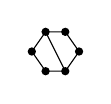
\begin{tikzpicture}[scale=.25]
      \node[vertex] (a) at (1,1) {};
      \node[vertex] (b) at (2,1) {};
      \node[vertex] (c) at (2.7,2) {};
      \node[vertex] (d) at (2,3) {};
      \node[vertex] (e) at (1,3) {};
      \node[vertex] (f) at (0.3,2) {};   
      
      \draw (1,1) -- (2,1) -- (2.7,2) -- (2,3) -- (1,3) -- (0.3,2) -- (1,1);
      \draw (2,1) -- (1,3);
    \end{tikzpicture}
    \caption{First candidate pattern\label{fig:iso1}}
  \end{minipage}
  \begin{minipage}{0.45\textwidth}
    \centering
    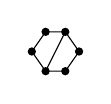
\begin{tikzpicture}[scale=.25]
      \node[vertex] (a) at (1,1) {};
      \node[vertex] (b) at (2,1) {};
      \node[vertex] (c) at (2.7,2) {};
      \node[vertex] (d) at (2,3) {};
      \node[vertex] (e) at (1,3) {};
      \node[vertex] (f) at (0.3,2) {};
 
      \draw (1,1) -- (2,1) -- (2.7,2) -- (2,3) -- (1,3) -- (0.3,2) -- (1,1);
      \draw (1,1) -- (2,3);
    \end{tikzpicture}
    \caption{Second candidate pattern\label{fig:iso2}}
  \end{minipage}
%  \caption{Possible patterns\label{fig:isomorphism}}
\end{figure}
\vspace{-1em}
Given the graph mining problem as specified in \textbf{Fig.} ~\ref{fig:ex1}, we have already established that \textbf{Fig.}~\ref{fig:iso1} is a valid pattern.
When we try to mine a second pattern, we might suggest a pattern as shown in \textbf{Fig.}~\ref{fig:iso2}.
A quick check, however, will show that there is a one-to-one mapping $f$ such that both $f$ as well as its inverse $f^{-1}$ preserve edges.
As a result, both candidate patterns are isomorphic, and thus only one should be accepted as a valid pattern.
%By Definition~\ref{def:canonicalForm} only one of these two patterns can be the canonical form, and therefore 
%Therefore, only one of these two candidate patterns should be accepted as a valid pattern.

\begin{definition} \textbf{Canonical Patterns}
A set of \emph{canonical patterns} is a set $\graphset{P}$ of graphs $\graph{P}_{1},...,\graph{P}_{n}$, such that for each pair of different elements (of \graphset{P}) $\graph{P}_{i}, \graph{P}_{j}$ holds that there does not exist an isomorphism between $\graph{P}_{i}$ and $\graph{P}_{j}$.
\end{definition}

%As evidenced from the definitions above, graphs are the main concept in the graph mining problem, and, when represented using a triple $\triple{E,l,c}$, graphs are inherent \emph{higher order objects}.
Graphs are the main concept in the graph mining problem, and, when represented using  tuples $\triple{V,E,l}$, graphs take the form of \emph{higher order objects}.
A set of graphs is equivalent to a set of triples.
The most straightforward representation of such a set would be a binary predicate.
%As the domains of this predicate range over predicates and functions, it is a higher order predicate.
In the graph mining context, the domains of this predicate range over predicates and functions, and therefore it is a higher order predicate.

It is very natural to consider and represent each graph as a \emph{coherent} ensemble of its own components: all characteristics (edges, labeling \ldots) of a graph are represented by separate entities or concepts, which are grouped together for each graph $\graph{G}$ in the tuple that describes it. We refer to this as the \emph{local coherence} of the graph representation.
Not only is this a very natural representation, this representation also makes it very explicit that all example graphs are \emph{independent}, and that the searches for homomorphisms between a pattern and example graphs are independent as well.
This motivates us to reason about graphs as locally coherent objects in our logical models as well.
However, the higher order representations needed to reason about graphs and sets of graphs as \emph{coherent} objects in our models are not yet fully supported by the logics of IDP and ASP.
In the following section discusses how to solve this using several modeling techniques.

%When reasoning about graphs, we see \emph{each graph} as a \emph{coherent} ensemble of its own components: 
%all characteristics (edges, labeling \ldots) of a graph are represented by separate entities or concepts, which are grouped together for each graph $\graph{G}$ in the triple that describes it.
%We refer to this as the \emph{local coherence} of the graph representation.
%As graphs are the main concepts we talk about in the graph mining problem, keeping this concept together leads to a natural KR representation.
%Furthermore, this locally coherent representation makes it very explicit that all example graphs are \emph{independent}, and that the search for a homomorphism between pattern and example graph is independent as well.
%A good solver can then discover this independence and leverage it to achieve better performance.

%A set of graphs, such as the argument of the cardinality operator above or the set of example graphs $\graphset{G}$, is equivalent to a set of triples.
%The most straightforward representation of such a set would therefore be a ternary predicate.
%As the domains of this predicate range over predicates and functions, this predicate would be a higher order predicate.

%These higher order representations for graphs and sets of graphs are not yet fully supported by the logics of IDP and ProB.
%In the following section we discuss how we deal with them.
%\todo{Illustrate local coherence with table}

